\documentclass[11pt,a4paper,twocolumn]{article}
\usepackage[T1]{fontenc}
\usepackage[utf8]{inputenc}
\usepackage{authblk}
\usepackage[english]{babel}
\usepackage{fancyhdr}
\usepackage{subfig}
\usepackage{floatrow}
\usepackage{float}
\usepackage{amsmath}
\usepackage{amssymb}
\usepackage{slashed}
\usepackage{graphicx}
\usepackage{todonotes}
\usepackage[toc,page]{appendix}
\usepackage{hyperref}
\usepackage{placeins}
\usepackage{cleveref}
\usepackage{multirow}
\usepackage{longtable}
\hypersetup{
	colorlinks,
	citecolor=purple,
	filecolor=black,
	linkcolor=blue,
	urlcolor=black
}
\usepackage{color}

\newcommand{\white}[1]{{\textcolor{white}{#1}}}



\newcommand*\samethanks[1][\value{footnote}]{\footnotemark[#1]}
\title{Transition Form Factor of the $\eta^{\prime}$ Meson with CLAS12}
\date{}

\author{M. C. Kunkel\thanks{Contact / Spokesperson, email: m.kunkel@fz-juelich.de} \qquad C. Hanhart \qquad D. Lersch\thanks{Co-Spokesperson, email: d.lersch@fz-juelich.de} \qquad J. Ritman \qquad \hspace{2.2cm} S. Schadmand \qquad X. Song \qquad A. Wirzba \\ \vspace{-0.3cm} \it Forschungszentrum J\"ulich, J\"ulich (Germany) \\ \vspace{0.3cm} V. D. Burkert \\ \it Jefferson Lab, VA (U.S.A.)  \\ \vspace{0.3cm} B. Kubis \\ \it University of Bonn, Bonn (Germany) \\ \vspace{0.3cm} L. Guo \\ \it Florida International University, FL (U.S.A.) \\ \vspace{0.3cm} M. J. Amaryan \\ \it Old Dominion University, VA (U.S.A.) \\ \vspace{0.3cm} I. J. D. MacGregor \qquad B. McKinnon \qquad G. Rosner \\ \it University of Glasgow, Glasgow (U.K.) \\ \vspace{0.3cm} W. J. Briscoe,  \\ \it The George Washington University, Washington, DC (U.S.A.) \\ \vspace{0.3cm} M. Hattawy \\ \it Argonne National Laboratory, IL  (U.S.A.) \\ \vspace{0.3cm} D. I. Glazier \\ \it Edinburgh University, Edinburgh, (U.K.) \\ \vspace{0.3cm} P. L. Cole \\ \it Idaho State University, ID (U.S.A.) \\ \  \\ \it \white{space space} and the CLAS Collaboration \newline \newline}


\renewcommand\Authands{, }
\fancypagestyle{firststyle}
{
	\fancyhf{}
	\renewcommand{\headrulewidth}{0pt}
	\fancyhead[C]{\Large A CLAS Proposal for PAC44}
}
\newlength{\figwidth}
\setlength{\figwidth}{0.9\columnwidth}

\newlength{\qfigheight}
\setlength{\qfigheight}{0.25\textheight}

\newlength{\hfigheight}
\setlength{\hfigheight}{0.5\textheight}

\def\piz{\pi^{0}}
\def\pizT{$\pi^{0} \ $}
 \def\pizDal{$\pi^{0} \rightarrow e^+e^- \gamma  $}
 
\def\etaT{$\eta $}
 \def\etaDal{$\eta \rightarrow e^+e^- \gamma  $}
 
\def\omT{$\omega  $}
 \def\omDal{$\omega \rightarrow e^+e^- \piz $}
 
\def\etaP{\eta^{\prime}}
\def\etaTP{$\eta^{\prime}  $}
 \def\etaPDal{$\eta^{\prime} \rightarrow e^+e^- \gamma  $}

 \def\phiT{$\phi  $}
 \def\phiDal{$\phi \rightarrow e^+e^- \eta  $}
 \def\phiDalT{\phi \rightarrow e^+e^- \eta  }
 
 \def\epemT{$ e^+e^-  $}
  \def\pipiT{$\pi^+\pi^-$}
 \def\epem{e^+e^-}

 \def\phiPR{$ep\to e'p \phi \rightarrow p e^+e^- \eta$}
 \def\etaPR{$ep\to e'p \etaP \rightarrow p e^+e^- \gamma$}
 
\def\grpath{figures}
\newcommand{\abbr}[1]{\textsc{\texttt{#1}}}
%%%% new commands and macros %%%%%%%%%%%%%%%%%%%%%%%%%%%%%%%%%%%%%%%%%%%
\newlength{\figwidth}
\setlength{\figwidth}{0.9\columnwidth}

\newlength{\qfigheight}
\setlength{\qfigheight}{0.25\textheight}

\newlength{\hfigheight}
\setlength{\hfigheight}{0.5\textheight}

\newcommand{\dedicationfont}{\fontencoding{T1}\fontfamily{anttlc}\fontseries{m}\fontshape{n}\fontsize{12}{15}\selectfont}

\newcommand{\acro}[1]{#1\@}
\newcommand{\abbr}[1]{\textsc{\texttt{#1}}}
\newcommand{\abbrlc}[2]{\textsc{\texttt{#1}}\texttt{#2}}
\newcommand{\desg}[1]{\texttt{#1}}
\newcommand{\todo}[1]{\textbf{\uppercase{\emph{#1}}}} %\textcolor{Orange}{#1}}}


%Some variables
%
%
\def\g12{\emph{g12}}

\def\G11{\emph{g11}}
\def\clas{\abbr{CLAS }}

\def\Lqcd{\mathcal{L}_{\mathtt{QCD}}}
\def\qfield{\psi}
\def\qbarfield{\overline{\psi}}

\def\grpath{/Users/Mike/phdthesis/MY_THESIS/figures/print}
\def\figures{/Users/Mike/phdthesis/MY_THESIS/figures/print}

\newcommand{\bank}[4]{$\mathtt{#1}^{#2}_{#3}\lbrack\mathtt{#4}\rbrack$}

\def\ith{$i$\textsuperscript{th}}

\def\um{{\text{$\mu$}}m}

%\def\coloronline{(Color online.)\ }
\def\coloronline{}

%%% particles
\def\p{\mathrm{p}}
\def\n{\mathrm{n}}
\def\Kp{\mathrm{K}^{+}}
\def\Km{\mathrm{K}^{-}}
\def\K0{\mathrm{K}^{0}}
\def\Y{\mathrm{Y}}
\def\epos{\mathrm{e}^{+}}
\def\eneg{\mathrm{e}^{-}}
\def\gamstar{\mathrm{$\gamma$}^{*}}
\def\piup{$\pi$}
\def\gammaup{$\gamma$}
%%% TAGGER and RF related times
\def\trf{t_{\mathtt{RF}}}
\def\ttag{t_{\mathtt{TAG}}}
\def\ttagrf{t_{\mathtt{TAG,RF}}}
\def\tprop{t_\mathrm{prop}}
\def\ttrigoffset{t_{\mathrm{trigger-offset}}}

%%% BEAM energy
\def\ebeam{E_{\mathrm{beam}}}

%%% Beta
\def\betasttof{\beta_{\mathtt{ST-TOF}}}
\def\betatof{\beta_{\mathrm{vtx}\mathtt{-TOF}}}
\def\betap{\beta_{p}}

%%% path lengths
\def\lst{\ell_{\mathtt{ST}}}
\def\ltof{\ell_{\mathtt{TOF}}}
\def\lsttof{\ell_{\mathtt{ST-TOF}}}

%%% raw subsystem times
\def\tst{t_{\mathtt{ST}}}
\def\ttof{t_{\mathtt{TOF}}}
\def\dtsttof{\Delta t_{\mathrm{ST-TOF}}}

%%% vertex times
\def\tv{t_{\mathrm{vtx}}}
\def\tvtagrf{t_{\mathrm{vtx}}(\mathtt{TAG_{RF}})}
\def\tvst{t_{\mathrm{vtx}}(\mathtt{ST})}

\def\adcst{\mathtt{ADC}_{\mathtt{ST}}}

\newcommand{\bra}[1]{\left<#1\right|}
\newcommand{\ket}[1]{\left|#1\right>}
\newcommand{\braket}[2]{\left<#1\middle|#2\right>}
\def\piz{$\mathrm{\pi^{0}}\ $}
\def\epem{$e^+e^-\ $}
% Document starts
\begin{document}
\maketitle
\clearpage
\section{Introduction}
Dalitz decays are radiative decays in which the photon is virtual and subsequently produces an electron positron pair, $P\rightarrow l^+l^-X$. Such decays serve as an important tool used to reveal the internal structure of hadrons and the interaction mechanisms between photons and hadrons. Furthermore, assuming point-like particles, the electromagnetic interaction is calculable within QED by the Kroll-Wada formula. Transition form factors quantify modifications of the point-like photon-meson vertex due to the transitions and interactions of the meson. The transition form factor can be characterized as $\left| F(q^2)\right|$, where $q^2$ is the square of the invariant mass of the lepton pair, and can be determined by comparing QED predictions to the experimentally measured rate. The goal of of this analysis is to determine the transition form factor for the $\etaP$ meson. This measurement will aide in limiting the largest uncertainty of the Standard Model prediction for hadronic quantum corrections in the muon anomaly.
\\
\indent From previous CLAS analyses using the g12 data set, it was shown that measurements of the time-like transition form factor were achievable, but without the statistical precision needed to be competitive. Therefore, we proposed to use the CLAS12 detector to measure the Dalitz decay channel of the reactions $ep\rightarrow e^{\prime}p\etaP$, where $\etaP \to e^+e^- \gamma$, through detection of the final state proton and $\etaP$ decay products. Preliminary studies using the CLAS12 simulation suite have shown that a beam time of 80 days, at full luminosity, will accumulate a data sample at least one order of magnitude larger in statistics than the most current $\etaP \to e^+e^- \gamma$ measurement and would yield a statistical uncertainty $\lesssim 0.5\%$. 

\indent Current measurements on the determination of the transition form factor have been performed in the space-like region ($\mathrm{q}^2<0$) in collider experiments. However, due to experimental limitations (e.g. $\pi^{\pm}$ contamination in lepton sample, low branching fractions, external conversion contamination), transition form factors in the time-like region ($\mathrm{q}^2>0$) have not yet been precisely determined. Recent measurements of the time-like transition form factor for $\etaP \to e^+e^- \gamma$ have been performed by the BESIII collaboration with insufficient statistical precision to distinguish between different theoretical approaches. 
\subsection{Motivation}
While very successful in many aspects, the Standard Model of particle physics (SM)
leaves a few important questions unanswered. On the one hand, it predicts
an amount of matter that survived annihilation after the Big Bang that is many orders
of magnitude less compared to what is observed. In addition, since masses
of matter particles appear as parameters in the SM, it does not provide any understanding
why the values of these masses span so many orders of magnitude.
In addition, within the SM, phenomena like Dark Matter and Dark Energy can not be explained.
These and some more 
issues suggest that there must be physics beyond the SM, and many experiments
world-wide hunt for signals of it. 

One of the currently most promising candidates to provide a signal for physics beyond the SM
is the muon anomaly. It is a low-energy observable, which
can be both measured and computed to high precision~\cite{Jegerlehner:2009ry,Blum:2013xva}.
``The anomaly is defined by $a_\mu = (g-2)/2$, where the Land\`e g-factor is the proportionality constant that relates the spin to the magnetic moment.
For the muon, as well as for the electron and tauon,
the anomaly $a$ differs slightly from zero (of order $10^{-3}$)
because of radiative corrections. In the Standard Model, contributions to the anomaly come from virtual `loops' containing photons and the known massive particles.''~\cite{miller} 
The present experimental value $a_\mu^{\rm EXP}= 1\ 165\ 920\ 89 (63)\times 10^{-11}$
comes from the BNL E821 experiment~\cite{Bennett:2006fi}.  This value
deviates from the SM prediction by about 3 standard
deviations $\Delta a_\mu^{({\rm EXP-SM})}= (287\pm 80)\times 10^{-11}$~\cite{Davier:2010nc} 
or $= (261\pm 78)\times 10^{-11}$~\cite{Hagiwara:2011af}, depending on how the leading-order
hadronic contributions are evaluated.  While this discrepancy
is not large enough to claim a failure of the SM, it is currently the largest
deviation of a SM prediction from an experimental observable. This
alone justifies the efforts currently taken to improve both the theoretical as well as the experimental value.
New measurements are planned within the next four years at 
Fermilab/USA~\cite{Grange:2015fou} and also at JPARC/Japan~\cite{Saito:2012zz}. The goal
of the measurements is to reduce the uncertainty by a factor of four. 
In parallel the SM prediction needs to be improved in accuracy 
by at least a factor of two to establish a deviation from the SM for the first time.


The largest uncertainty of the SM prediction comes from
the hadronic quantum corrections~\cite{Jegerlehner:2009ry}.
At the level of accuracy that is relevant at the moment the hadronic
contributions can be split up into the hadronic vacuum polarization
(HVP), displayed on the left-hand side of figure \ref{fig:gm2}, and the
hadronic light-by-light scattering (HLbL), displayed in the middle of
Fig.~\ref{fig:gm2}. The most important contribution to the latter
comes from the pseudoscalar pole contributions, displayed explicitly on the right-hand 
side of Fig.~\ref{fig:gm2}. For those one expects that the contribution
should be largely saturated by the lightest exchange particles, namely the 
$\pi^0$, the $\eta$ and the $\eta'$. 
%
\begin{figure}[!h]
	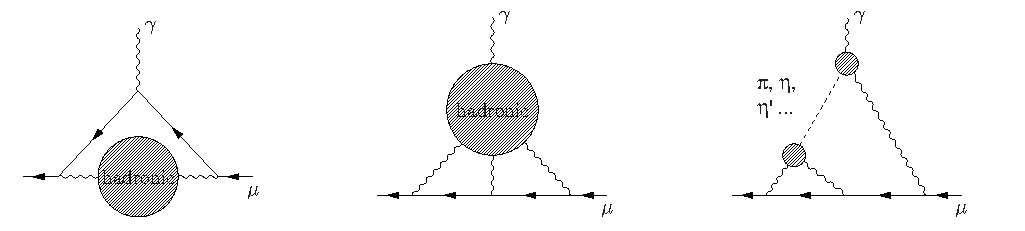
\includegraphics[keepaspectratio,width=1.\textwidth]{figures/hadronicgm2.pdf}
	\caption{Hadronic contributions to $a_\mu$: hadronic vacuum polarization (left diagram), 
		hadronic light-by-light scattering (middle), pion-pole contribution to hadronic light-by-light scattering (right). Full lines with an arrow denote muons, wiggly lines photons, the dashed line a pseudo-scalar meson and shaded blobs a non-pointlike hadronic substructure. The upper blob in the right diagram corresponds to Fig.~\ref{fig:piz.dalitz}, while the lower blob corresponds to the double Dalitz decay. 
	}
	\label{fig:gm2}
\end{figure}

Concerning the SM prediction for $a_\mu$ HLbL is suppressed relative to HVP by one power of the electromagnetic
fine structure constant~\cite{Jegerlehner:2009ry,Bijnens:2007pz}.  
Unfortunately at present it is not possible to straightforwardly 
calculate the contributions shown in Fig.~\ref{fig:gm2} 
from first principles analogously to, e.g., the QED corrections, since
both processes concern low-energy corrections,
i.e.\ non-perturbative physics. Thus the prime candidate for a SM
calculation of hadronic corrections seems to be lattice QCD~\cite{Gattringer:2010zz}. 
However, it is not expected that lattice QCD
results for HPV will reach the required accuracy in the foreseeable future.
For the HLbL only preliminary lattice-QCD calculations have been reported~\cite{Blum:2014oka}.  
In view of the challenges to determine
a four-point function that includes in addition disconnected diagrams
it is not clear yet when a profound lattice calculation with
controlled uncertainties and a reliable error estimate will be
available.

Fortunately there is an alternative way to quantify hadronic corrections. It requires both
theoretical as well as experimental efforts:
Dispersion theory provides a link between particular hadronic cross sections
and $a_\mu$---for a discussion of the HVP in this context see Ref.~\cite{Jegerlehner:2009ry}, while 
for HLbL we refer to Refs.~\cite{Colangelo:2014dfa,Pauk:2014rfa,Colangelo:2014pva,Colangelo:2015ama}.  
In particular for the latter contribution it allows one to calculate from the transition
form factors of the kind $\pi^0$, $\eta$, $\eta'\to \gamma^*\gamma^*$ 
the corresponding piece for the meson pole contribution as displayed in the
right most diagram of Fig.~\ref{fig:gm2}.
The measurements proposed here provide important information towards
the necessary input needed for the evaluation of the HLbL contribution, since
$\eta'\to \gamma^*\gamma$ gives the single off-shell form factor of the $\eta'$
and $\phi\to \eta\gamma$ additionally provides information on the isoscalar
piece of $\eta\to \gamma^*\gamma$ in a different kinematic regime.
Additional information on the  $\eta$ and
$\eta'$ form factors can be found from the dispersive methods outlined in
Refs.~\cite{Adlarson:2011xb,Stollenwerk:2011zz,Hanhart:2013vba,Kubis:2015sga,Xiao:2015uva}.
It  appears to be realistic that this joined effort of theory and experiment
will provide the improvements necessary to push the SM calculation towards
the required accuracy. For the $\etaP$ pole contribution a precision of 15\% on the HLbL correction are feasible.~\cite{Nyffeler}.

\section{Kinematics of Decays}\label{sec:kinematics}
The channel proposed to be studied is 
\begin{align}
e(k)+p(p)\to e'(k') + p'(p') +\etaP(\nu) \label{eq:etaP} 
\end{align}
where $k$, $k'$, $p$, $p'$ are the four–momenta of the incident lepton, outgoing lepton,target proton and scattered proton respectively. The virtual photon in the production is defined as $q=k-k'$ with energy $v = \frac{pq}{m_p} = E - E'$. The quantity $\etaP(\nu)$ is the electro-produced meson. Production mechanisms of similar mesons have been already proposed in previous proposals~\cite{clas.proposal.eta,clas.proposal.phi} and are scheduled to run in conjunction with RunGroupA, the same run group requested for in this proposal.
The main decays studied for this proposal are:
\begin{align}
\etaP \rightarrow \gamma \gamma \to e^+e^- \gamma \label{eq:etaPconv} \\
\etaP \rightarrow \gamma \gamma^\star \to \gamma e^+e^- \label{eq:etaPDal} 
\end{align}
i.e. when a pseudoscalar meson, $P_p$($\eta'$), decays via two photons (Eq.~\ref{eq:etaPconv}) and one photon converts into an \epemT \ pair due to E.M. processes through matter, this is conventionally known as external conversions. The Dalitz decay(Eq.~\ref{eq:etaPDal}), or internal conversion, is when the $P_p$($\eta'$) decays via a real photon and a virtual photon, which decays into an \epemT \ pair.
Figure~\ref{fig:piz.alldecay} illustrates the Feynman diagrams for the pseudoscalar ``two photon decay'' and  ``Dalitz decay''.
%Table~\ref{tab:pi0}. Figure~\ref{fig:piz.alldecay} illustrates the Feynman diagrams for the ``Two photon decay'' and the ``Dalitz decay''.
\begin{figure}[h!]\begin{center}
		\subfloat[Feynman Diagram of $\etaP$ Two Photon Decay][]{ %Feynman diagram of $\etaP$ two photon decay
			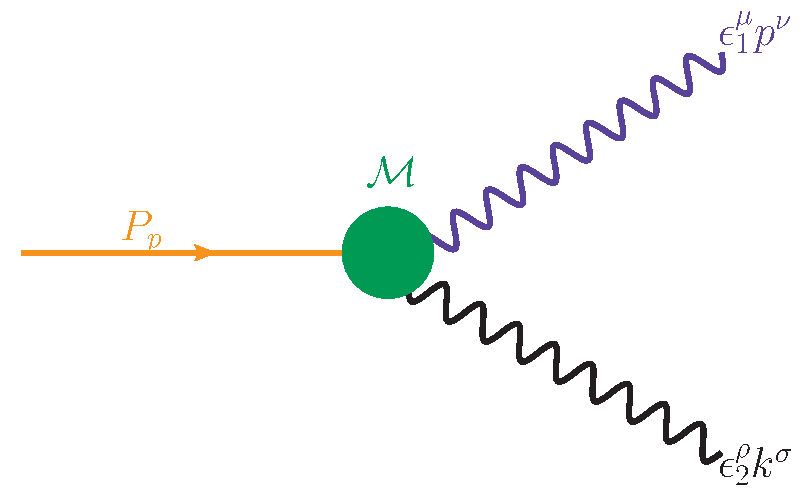
\includegraphics[width=0.4\columnwidth,height=0.55\qfigheight]{figures/psudoscalar_gammagamma.pdf}\label{fig:piz.gamgam}
		}
		\quad
		\subfloat[Feynman Diagram of $\etaP$ Dalitz Decay][]{ %Feynman diagram of $\etaP$ Dalitz decay
			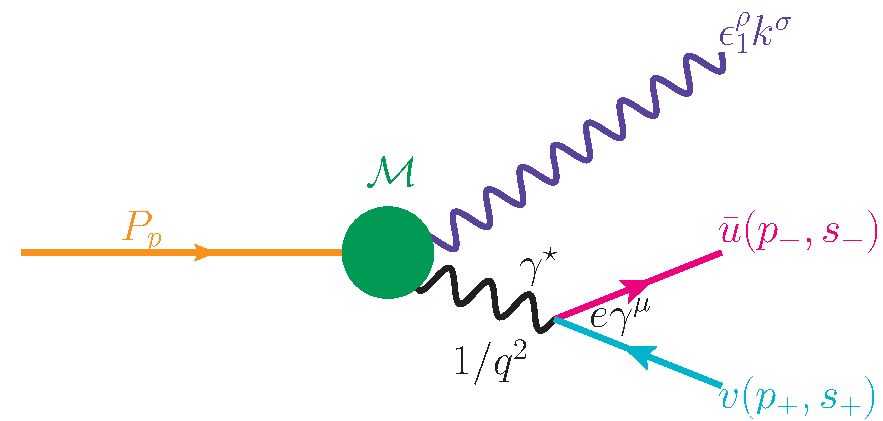
\includegraphics[width=0.45\columnwidth,height=0.55\qfigheight]{figures/psudoscalar_dalitz.pdf}\label{fig:piz.dalitz}
		}
		\caption[Feynman diagram of $P_p$($\etaP$) two photon decay and Dalitz decay]{\label{fig:piz.alldecay}Feynman diagram of $P_p$($\etaP$) two photon decay~\subref{fig:piz.gamgam}, $\epsilon_1$ and $\epsilon_2$ are the polarizations, $p$ and $k$ are 4-momenta of the photons.  Feynman diagram of $P_p$($\etaP$) Dalitz decay~\subref{fig:piz.dalitz}, the variable $s_\pm$ are the spin helicities of the outgoing leptons $l^\pm$ with 4-momenta $p_{\pm}$ and $\epsilon$ is the polarization of the outgoing photon with 4-momenta $k$. In both diagrams $\mathcal{M}$ is the form factor.}
	\end{center}\end{figure}
	\FloatBarrier
	\subsection{The Dalitz Decay}
	The Dalitz decay of mesons is dependent on the spin of the meson. For a pseudoscalar meson ($P$), the decay rate can be expressed as:
	\begin{align*}\label{eq:eegff.finalkroll_II}
	\frac{d\Gamma_{P_{\epem \gamma}}}{\Gamma_{P_{\gamma\gamma}} dq^2} = & \frac{2 \alpha}{3 \pi} \frac{1}{q^2} \left( 1- \frac{q^2}{m_p^2}\right)^3 \times \\ &\left( 1+ \frac{2m_l^2}{q^2}\right) \left( 1- \frac{4m_l^2}{q^2}\right)^{\frac{1}{2}} 
	\end{align*}
	which is the Kroll-Wada equation found in~\cite{KrollWada,landsberg}.
	An example of QED expectation for \etaTP  \ is shown in Fig.~\ref{fig:dalitz_compare}.
	\subsection{Form Factor}
	It has been experimentally observed that the shape of the dilepton mass spectrum deviates significantly from the QED predictions, displaying a rise at larger dilepton mass. Therefore, the form factor ${M}_P(p^2,k^2=0)$ or ${M}_P(p_{1}^2,p_{2}^2)$  can be written as follows:
	\begin{align}
	{M}_P \to {M}_P' \times \left|F(q^2)\right| \ ,
	\end{align}
	where $M_P'$ is the decay constant of two photons or $\eta$ photon, while $\left|F(q^2)\right|$ is called the transition form factor, which defines the electromagnetic space structure of the meson. According to that, the $\etaP \to e^+e^- \gamma$ decay rate modifies as;
	\begin{align*}\label{eq:eegff.final}
	\frac{d\Gamma_{\epem \gamma}}{\Gamma_{\gamma\gamma} dq^2} = & \frac{2 \alpha}{3 \pi} \frac{1}{q^2} \left( 1- \frac{q^2}{m_p^2}\right)^3 \left( 1+ \frac{2m_l^2}{q^2}\right) \times \\ & \left( 1- \frac{4m_l^2}{q^2}\right)^{\frac{1}{2}} \left|F(q^2)\right|^2 \ ,
	\end{align*}
	First observations were described with standard vector meson dominance (VMD) where the virtual photon can stem from intermediate vector mesons. 
	The value of $\left|F(q^2)\right|$ can be directly measured by comparing QED predictions to the measured rate~\cite{landsberg}. 
	\begin{align}
	\frac{d\Gamma(A\to B+l^+l^-)}{dq^2 \Gamma(A\to B\gamma)} = \left[\frac{d\Gamma}{dq^2}\right]_{\text{QED}} \cdot \left | F(q^2) \right |^2 
	\end{align}
	or by performing a line shape analysis on the $l^{+}l^{-}$ invariant mass using assumptions on the structure of $\left|F(q^2)\right|$. One such assumption for $\left|F(q^2)\right|$ is the dipole approximation from the VMD model, which can be parametrized as:
	\begin{align}\label{TFFbitch}
	F(q^2) = \frac{1}{1-q^2/\Lambda^2} 
	\end{align}
	where the parameter $\Lambda$ corresponds to the mass for the effective contributing vector meson.	
	The slope of the transition form factor, $b$, is defined as:
	\begin{align}
	b \equiv \frac{dF}{dq^2}|_{q^2=0} \label{eq:tffslope}.
	\end{align}
	and characterizes the intrinsic spatial charge radius for the $\etaP$ meson. Several theoretical approaches have been developed to describe the transition form factor and are listed in Tab.~\ref{tab:theory}.
	\begin{table}[h!]
\begin{minipage}{\textwidth}
\begin{center}

\caption[Theoretical approaches]{\label{tab:theory}Theoretical approaches to describe the transition form factor \vspace{0.75mm}}

\begin{tabular}{c|c}

\hline
Approach & slope parameter ($b_{\eta'}$) \\
\hline
Dispersion & $1.53^{+0.15}_{-0.08} \mathrm{GeV^{-2}}$ \\
Chiral Perturbation &  $1.6 \mathrm{GeV^{-2}}$ \\
VMD &  $1.45 \mathrm{GeV^{-2}}$ \\
\hline \hline
\end{tabular}


\end{center}
\end{minipage}
\end{table}
	\begin{figure}[h!]\begin{center}
			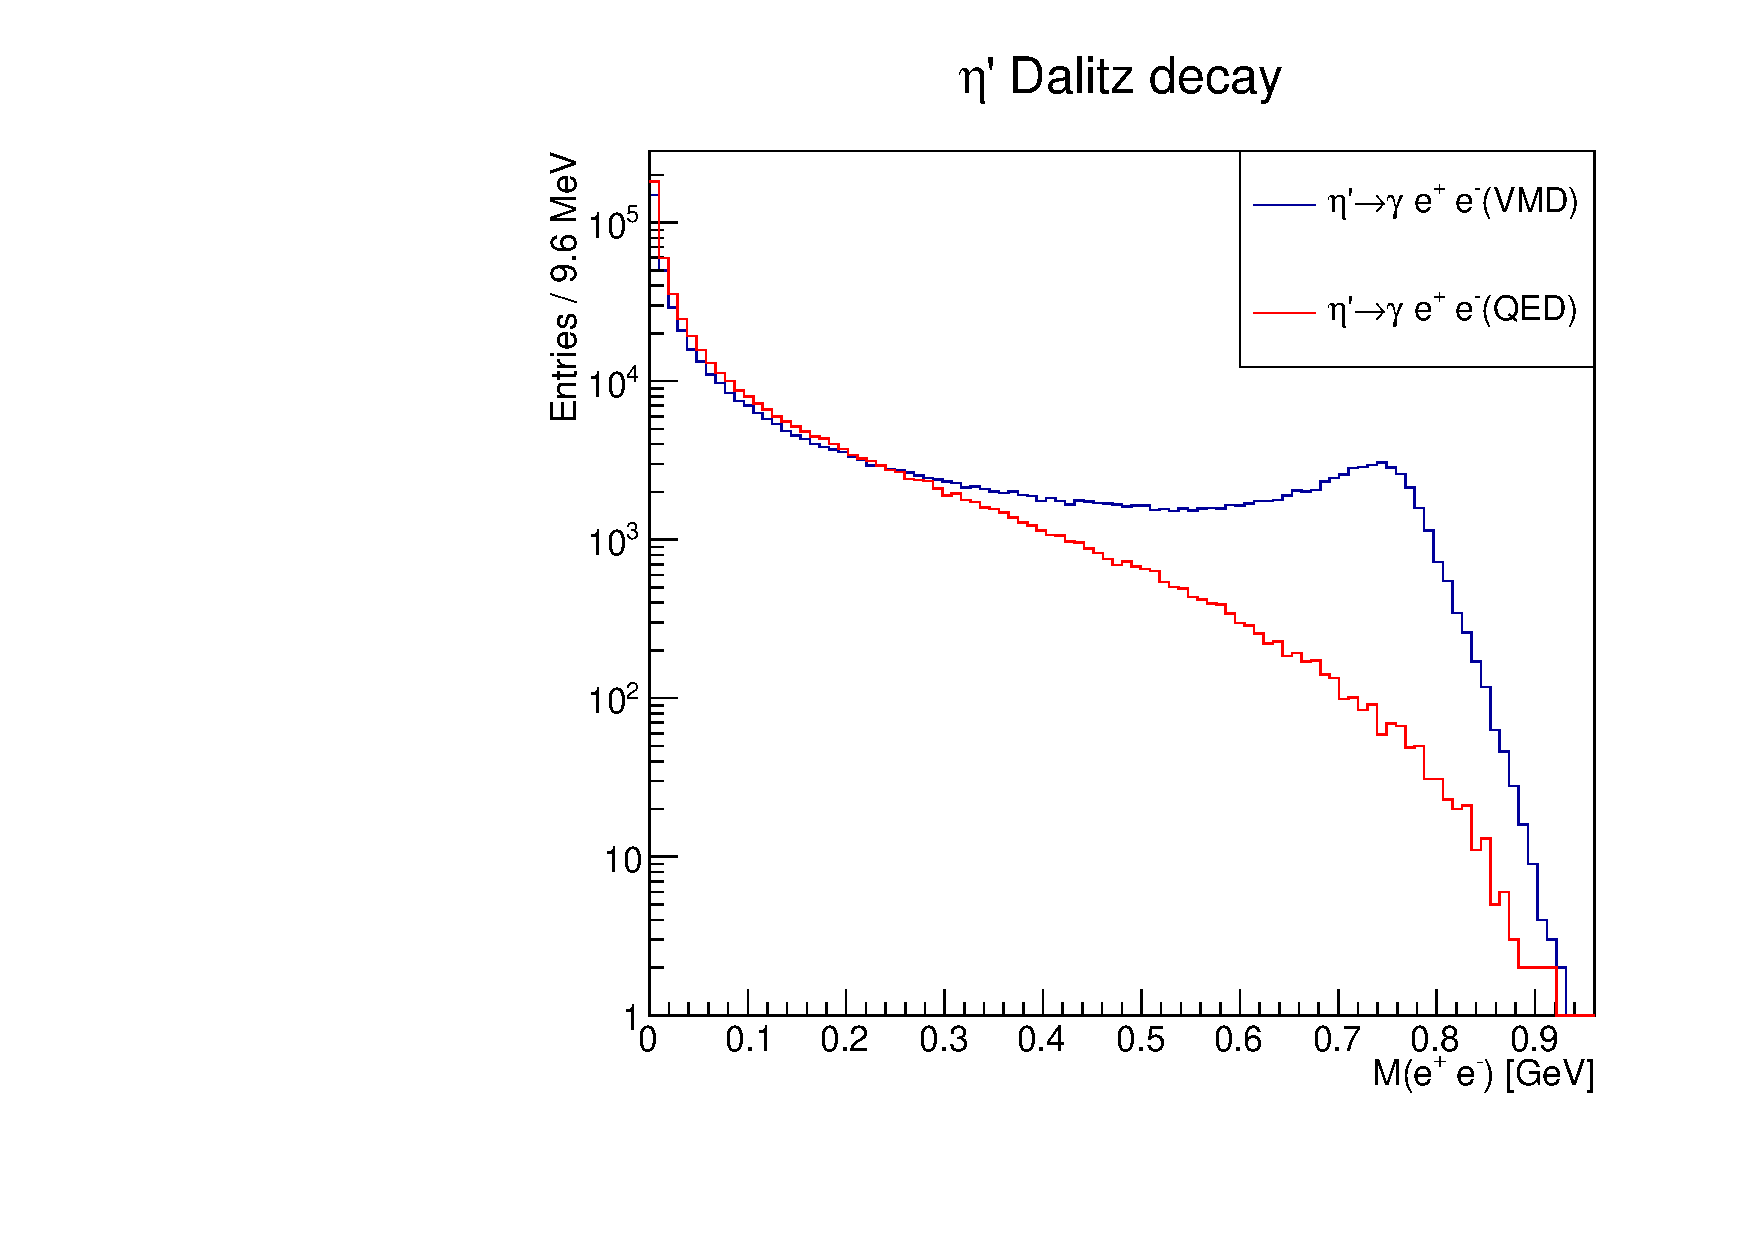
\includegraphics[width=0.8\columnwidth,height=1.0\qfigheight]{figures/etaP_Dalitz_QED_FF_comparePlot.pdf}\label{fig:etap_dalitz_conpare}
			\caption[Dalitz  for \etaTP \ and $\phi$]{\label{fig:dalitz_compare}Example of Dalitz spectra for \etaTP \ using only QED(red) and the deviation from QED using the VMD parameterization(blue) with 500K Dalitz events generated. }
		\end{center}\end{figure}
	
\FloatBarrier
\section{Proposed Measurement}\label{sec:measurement}
\subsection{Simulation and Reconstruction}
\indent The production of \etaTP \ was weighted by photo-production differential cross-sections, $\frac{d\sigma}{d\Omega}(v,\cos\theta_{cm})$, published in~\cite{Williams}, and $Q^2$. Where $v$ is the virtual photon energy, $\cos\theta_{cm}$ is the production angle in the center-of-mass frame of the system and the virtual photon flux as a function of $Q^2 = -(k-k')^2$. This was done to achieve a quasi realistic model of the production. The \epemT \  decay spectrum, of each meson, was weighted via the VMD model (including QED predictions). Another simulation was performed using a flat $M(\epem)$ distribution (No QED, No VMD) to analyze any effects of the model on the \epemT acceptance. The analysis showed that the acceptance, in $M(\epem)$, was independent of the decay model until $M(\epem)\to M_{\etaP} $, see Fig.\ref{fig:counts}.
\subsubsection{Particle Identification}
The $\etaP$ meson have pion decay modes, which are orders of magnitude greater than the Dalitz decay. For example, the ratio $\Gamma_{\pi^+\pi^-\gamma} / \Gamma_{e^+e^- \gamma} $ is $ 6.2\cdot 10^2$. 
Electrons/positrons will be identified by using the information from the High Threshold Cherenkov counters (HTCC) and Electro-magnetic Calorimeters (PCAL+EC). The expected $e^\pm/\pi^\pm$ rejection factor for single particles (p<4.9~GeV) is $10^3$ for the HTCC, while the PCAL+EC can provide an additional factor of $10^2$. Combining both methods yields a $e^\pm/\pi^\pm$ rejection factor of $10^5$ which results in a $e^+e^-/\pi^+\pi^-$ rejection factor of $10^{10}$. Therefore, the amount of $\pi^+\pi^-$ background in the $M(\epem)$ spectrum will be $\approx 6.2\cdot 10^2/10^{10} = 6.2\cdot10^{-8}$. A detailed explanation of particle identification for \epemT \ pairs can be found in~\cite{clas.proposal.jpsi}.
\FloatBarrier
\subsection{Calculating the Expected Yield}\label{sec:yield}						
The rate for mesons in electro-production where the scattered electron is left undetected (W=1.9-2.7~GeV) is $\sim 80\,\rm{kHz}$~\cite{Sargsyan}. This rate needs to be scaled down by the production cross-section ($\sigma(W)$) in order to achieve the corresponding rate for $\etaP$ production. 
A plot of Eq.~\ref{etaPRate} is shown in Fig.~\ref{fig:EtaPRate} (left y-axis). The total $\etaP\rightarrow\epem\gamma$ rates per 80 days, and as a function $W$, is calculated by multiplying Eq.\ref{etaPRate} with the product of the average detection efficiency $\epsilon\approx 5\%$ as well as the branching fraction $\mathcal{BR} = 4.69\cdot10^{-4}$~\cite{BESIII} for $\etaP\rightarrow\epem\gamma$. The corresponding plot is shown in Fig.~\ref{fig:EtaPRate} (right y-axis). The total number $N_{tot}$ of expected $\etaP\rightarrow\epem\gamma$ events after 80 days of measurement is given by the integral of Fig.~\ref{fig:EtaPRate} over $W$. This leads to the expected yield:
						
\begin{align}
	N_{tot} &= \int\limits_{1.9\,\rm{GeV}}^{2.8\,\rm{GeV}} \Big[ {\color{red}{N(W)_{\etaP\rightarrow\epem\gamma\text{ / 80 Days }}}} \Big]dW   \\ & =  \mathrm{\frac{28,200 \ events}{80 Days}}
\label{yield}
\end{align}
						
						
\begin{figure}[h!]\begin{center}
\includegraphics[width=1.0\figwidth,height=1.4\qfigheight]{figures/Total_rates.pdf}\\
\caption[etaP rates]{\label{fig:EtaPRate}{Total $\etaP$ production rate per 80 days (left y-axis) and total $\etaP\rightarrow \epem\gamma$ rates per 80 days (right y-axis) as a function of $W$. }}
\end{center}\end{figure}
							
\begin{figure}[h!]\begin{center}
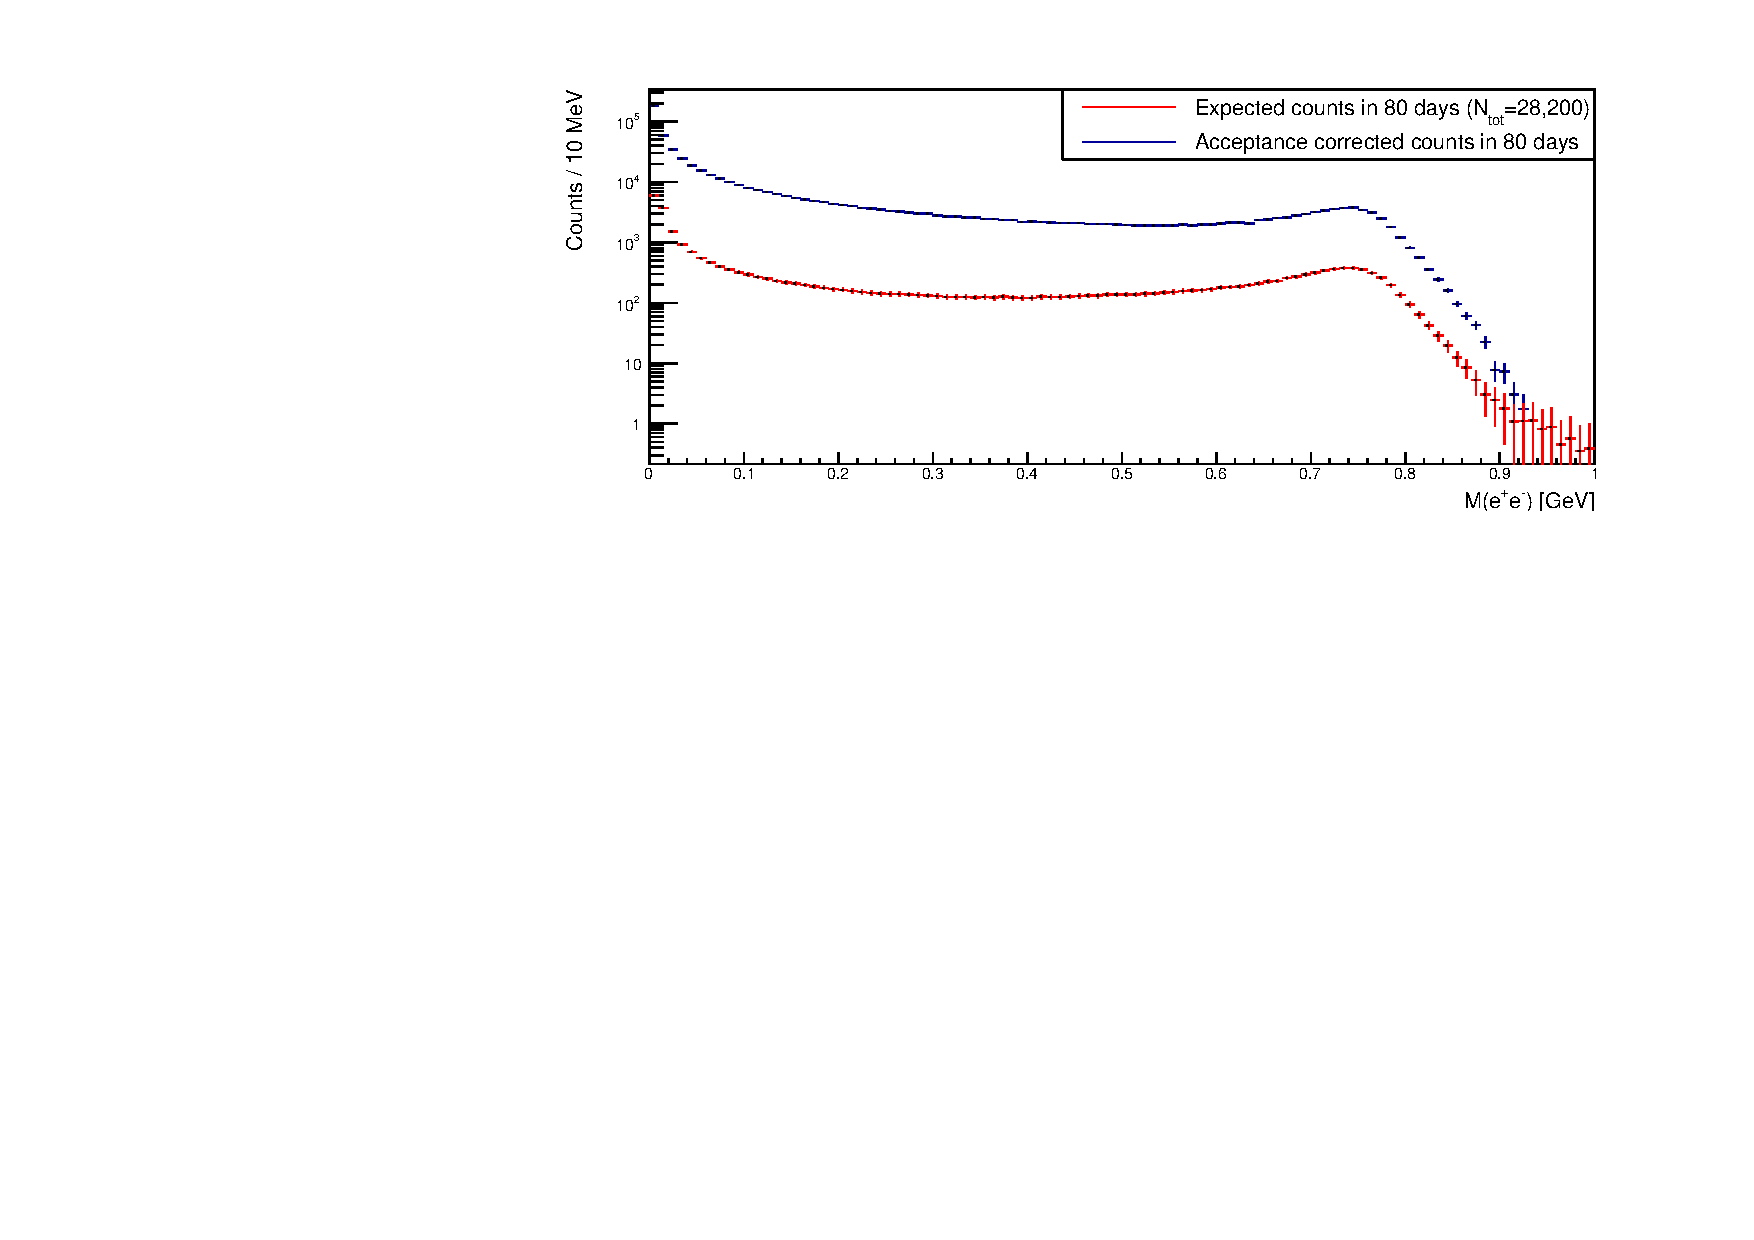
\includegraphics[width=\figwidth,height=1.3\qfigheight]{figures/counts.pdf}
\caption[Acceptance as a function of $M(\epem)$]{\label{fig:counts}{(Color Online)Expected yield as a function of $M(\epem)$.}}
\end{center}\end{figure}
								
\begin{figure}[h!]\begin{center}
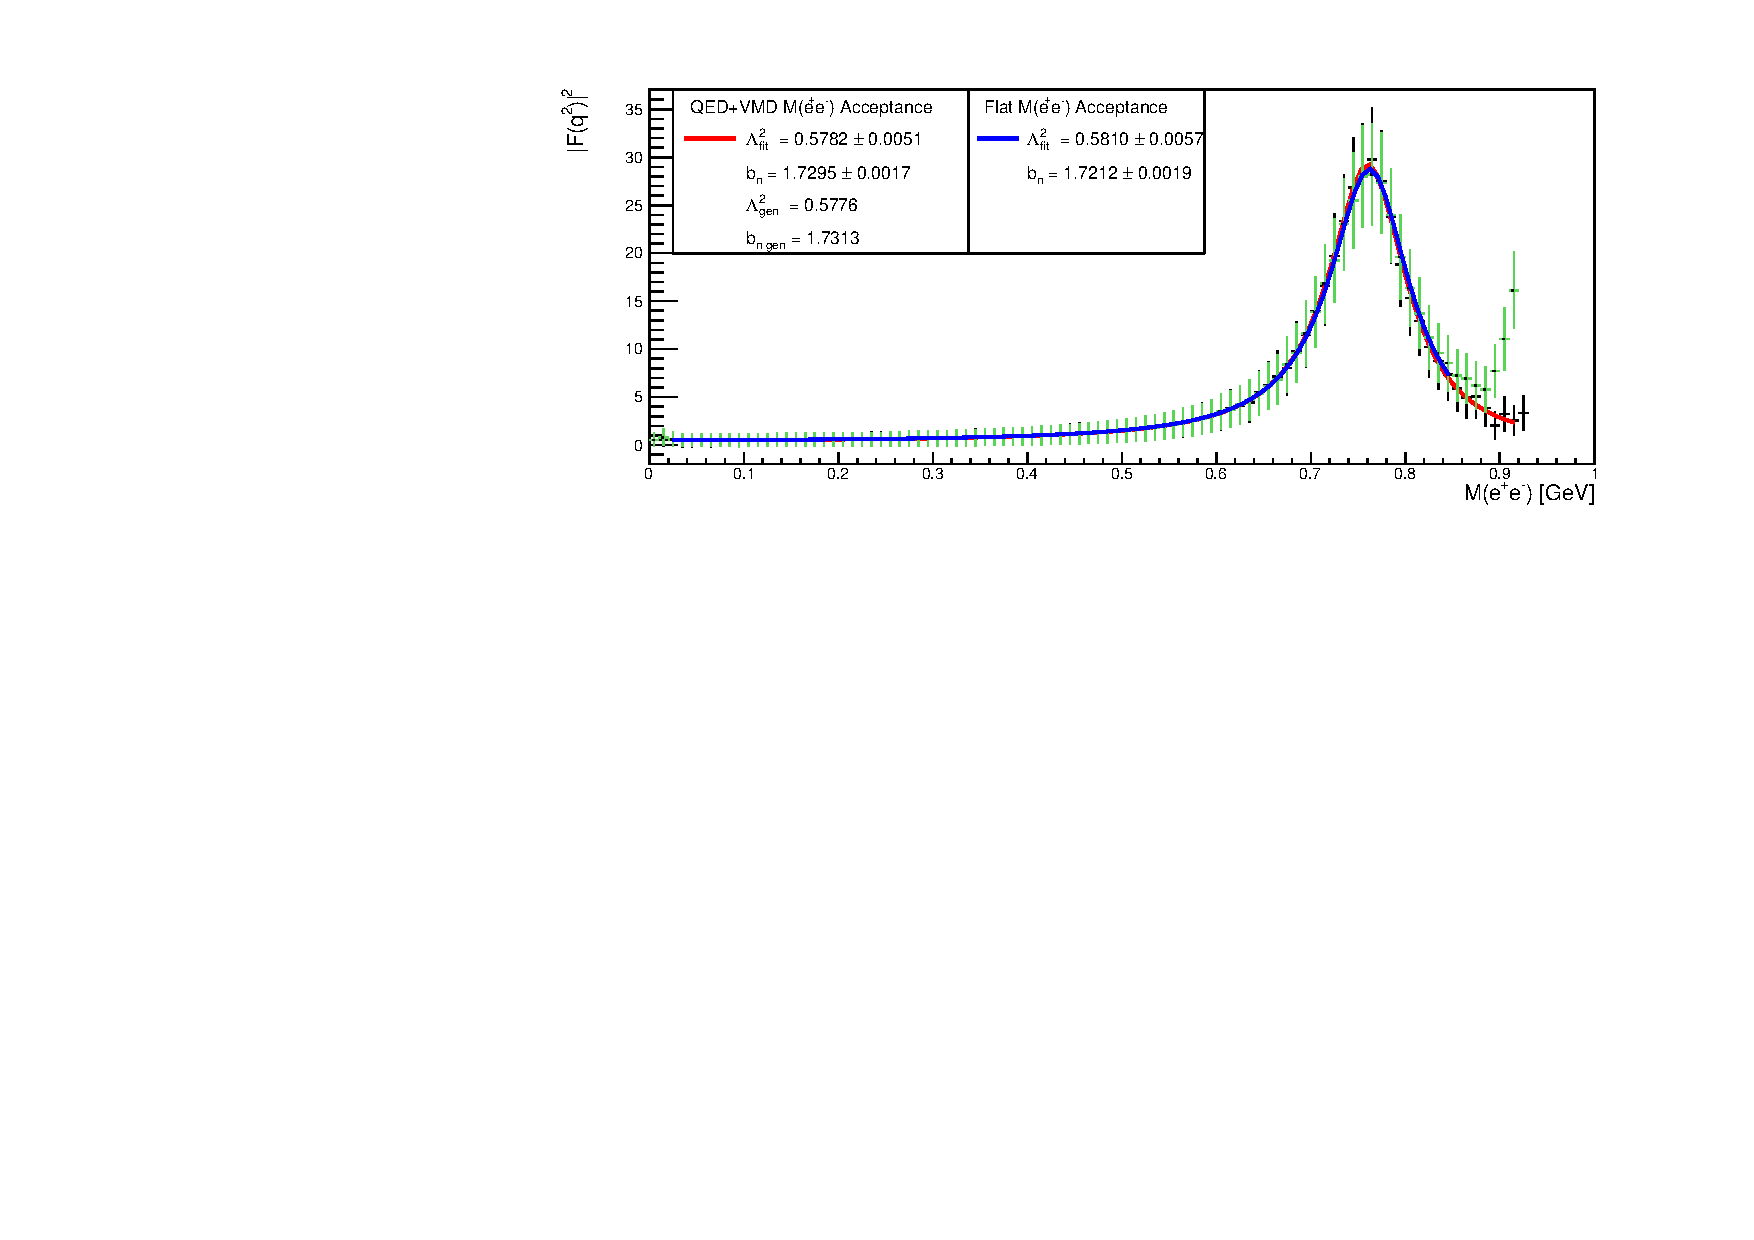
\includegraphics[width=\figwidth,height=1.3\qfigheight]{figures/result.pdf}
\caption[TFF as a function of $M(\epem)$]{\label{fig:results}{(Color Online)$\left|F(q^2)\right|^2$ as a function of $M(\epem)$ using two acceptance models. (black points) QED+VMD $M(\epem)$ acceptance model. (green points) Flat $M(\epem)$ acceptance model. The solid lines represent a fit using Eq.~\ref{TFFbitch} to the data points.}}
\end{center}\end{figure}
									
\FloatBarrier
From Fig.~\ref{fig:counts} the QED normalized spectrum can be deduced and is shown in Fig.~\ref{fig:results}. Both acceptance models (i.e. flat and QED+VMD) are used to determine the transition form factor. It is shown that there exists a systematic uncertainty depending on the chosen acceptance model. However, the final calculation on the slope parameter or the TFF shows a negligible impact of this uncertainty. Regardless of the acceptance model, it is shown in Fig.~\ref{fig:results} that the accumulated statistics collected by CLAS12 allow for a precision of each parameter $\lesssim 0.5\%$. 
\subsection{Expected Systematic Uncertainties}
The major sources of systematic uncertainties are the acceptance and particle identification. The di-lepton acceptance uncertainty is estimated to be $\lesssim$ 5\% which was observed in former CLAS experiments. The lepton identification uncertainty will arise from the performance of the HTCC, PCAL and EC. From simulation studies performed for this proposal, all leptons and final state photons are detected within the geometric space of the PCAL+EC with hit coincidences in both. Furthermore, all leptons, within a few percent, that were detected in the PCAL+EC were also detected in the HTCC. Further systematics from pion contamination are mitigated by the pion rejection factor described above. Systematics related to external photon conversion are minimal due to the  1~mm resolution of the primary vertex given by the Silicon Vertex Tracker (SVT). Any Bethe-Heitler contributions are negligible when utilizing and exclusive meson reconstruction scheme. To estimate the systematic uncertainty on the expected slope parameter and TFF a 5\% increase in di-lepton acceptance as a function of $M(\epem)$ was applied, i.e.
\begin{align}
\epsilon_{new} = \epsilon \cdot (1+0.05 \cdot M(\epem)) \label{eq:sys} 
\end{align}
As seen in Fig.~\ref{fig:EPEMsys} the systematic arising from the di-lepton uncertainty can be calculated to be:
\begin{align}
	b_{n}^{sys} =0.0497 \% \\
\Lambda^{2}_{sys} = 0.0494 \%\ .
\end{align}
\begin{figure}[h!]\begin{center}
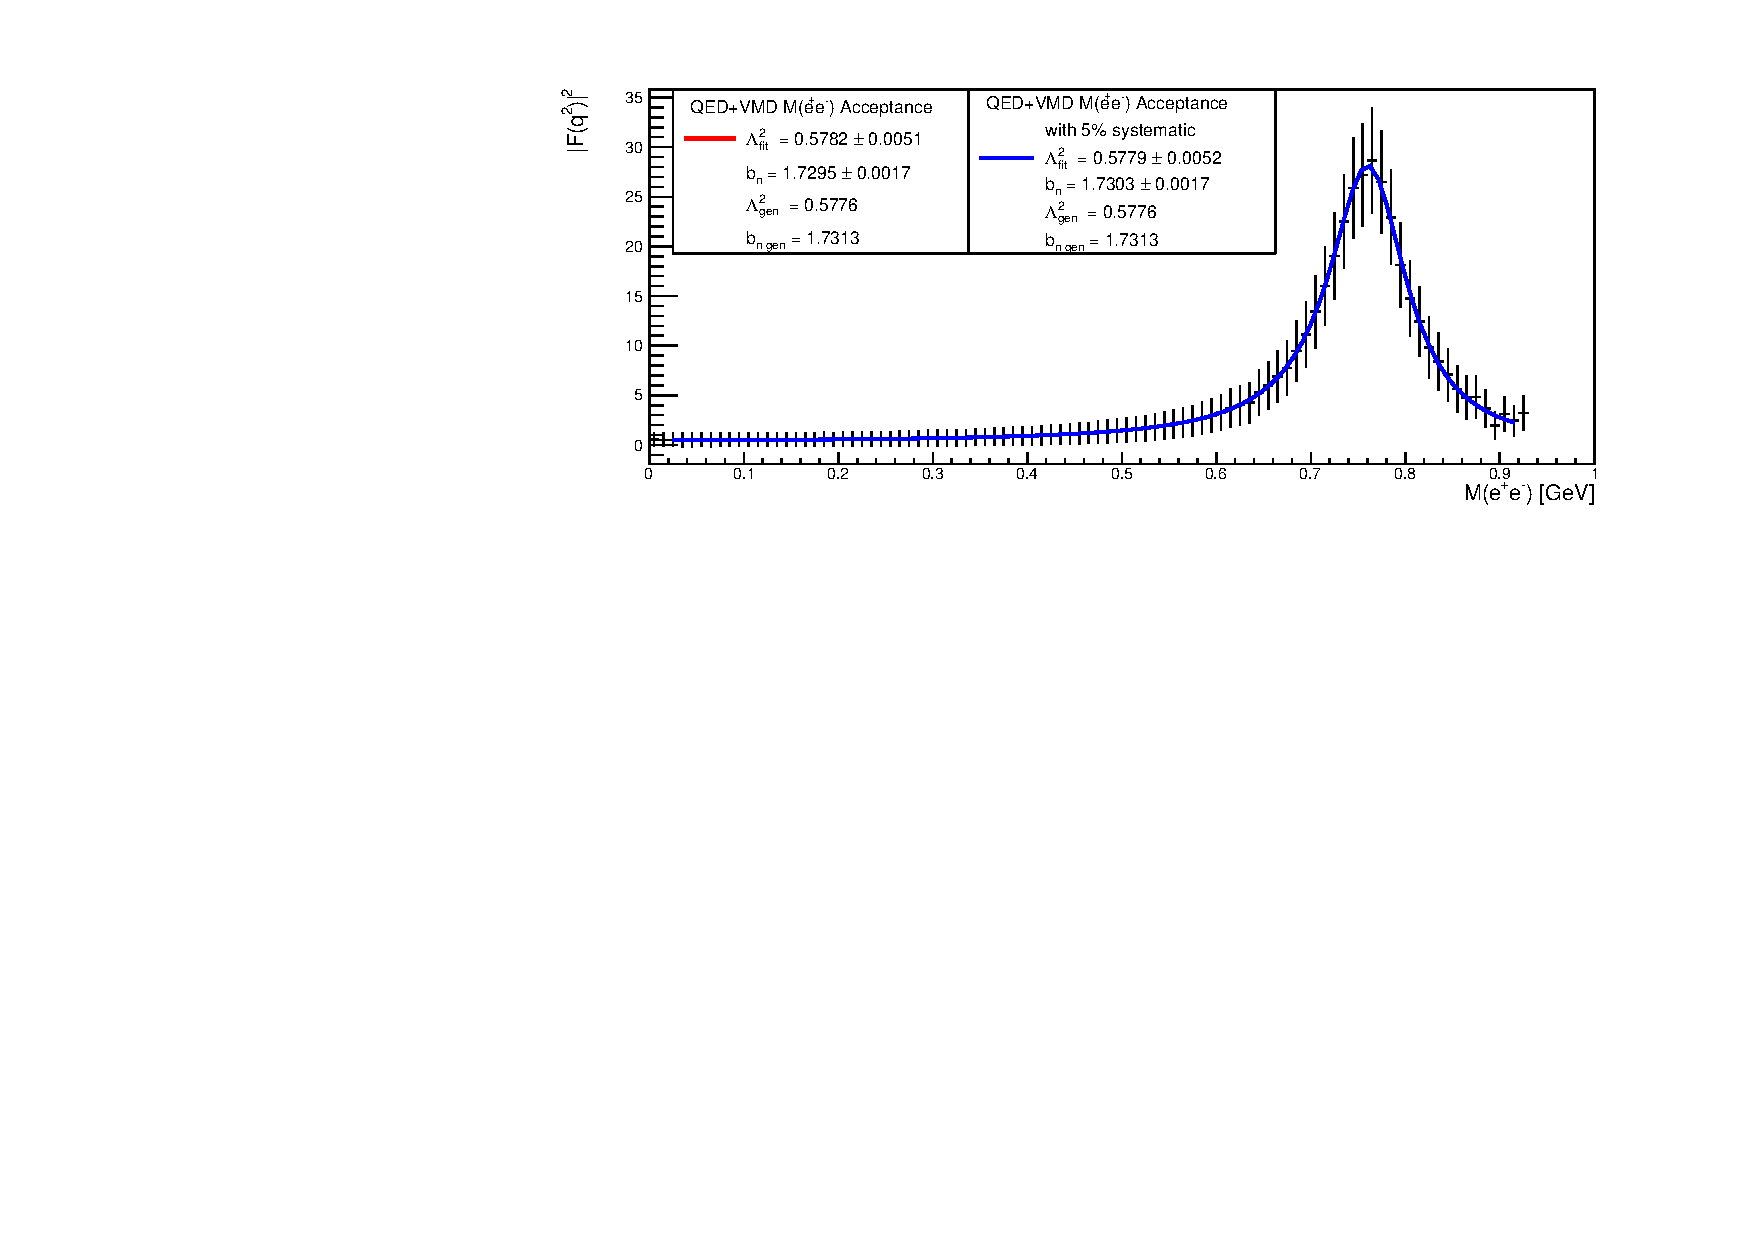
\includegraphics[width=\figwidth,height=1.3\qfigheight]{figures/sys.pdf}
\caption[Acceptance as a function of $M(\epem)$]{\label{fig:EPEMsys}{(Color Online)Expected yield as a function of $M(\epem)$ with a gradual 5\% increase in $M(\epem)$ acceptance .}}
	\end{center}\end{figure}
\FloatBarrier
\section{Approved Beam Time Request}\label{sec:beamrequest}
With this proposal and beam time request, we asked to run for 80 days parallel with the beam time already approved for Run-group A. The 80 day request was approved. This request will provide a competitive data sample of $\etaP \to \epem \gamma$. 
\section{Conclusion}
Compared to current experimental uncertainties of 10\% and differences in theoretical approaches of $\approx$ 10\%~\ref{tab:theory}, this approved proposed measurement by CLAS12 would not only be in the position to decisively discriminate between the theoretical predictions, but also pin down one of the largest uncertainties to the muon g-2 anomaly.								

\clearpage
\phantomsection 
\addcontentsline{toc}{section}{BIBLIOGRAPHY}
\bibliographystyle{unsrt}
\bibliography{Meson}	

\end{document}